\chapter{Stand van zaken}
\label{ch:stand-van-zaken}

% Tip: Begin elk hoofdstuk met een paragraaf inleiding die beschrijft hoe
% dit hoofdstuk past binnen het geheel van de bachelorproef. Geef in het
% bijzonder aan wat de link is met het vorige en volgende hoofdstuk.

% Pas na deze inleidende paragraaf komt de eerste sectiehoofding.

In dit hoofdstuk wordt de stand van zaken besproken wat tabeldetectie en tabelstructuuranalyse betreft. Er wordt besproken waarom tabellen belangrijk zijn in de huidige informatiewereld, wat er bedoeld wordt met tabeldetectie en structuuranalyse, waar de uitdagingen hierbij zich bevinden en tenslotte wordt er in detail de verschillende technieken besproken die ontwikkeld werden om tabellen te kunnen detecteren en analyseren, met hun voor- en nadelen.

\section{Tabulair data}
\label{sec:tabulair-data}

\subsection{Definitie}
\label{subsec:definitie-tabulair-data}

Zoals \textcite{Zanibbi2003} het aangeeft, is een tabel een vorm van visualiatie dat men gebruikt om ermee data op te zoeken en te vergelijken. Meer specifiek geeft, volgens \textcite{Zanibbi2003}, een tabel indexeringschema's weer voor relaties. Een relatie heeft een verzameling van $\eta$ \glspl{tupel}, die de domeinen of dimensies van de relatie genoemd worden.

De dimensies kunnen d.m.v. verschillende combinaties van rijen en kolommen opgesteld worden, waardoor verschillende tabelopstellingen exact dezelfde informatie op verschillenden manieren kunnne weergeven. Dit kan gedemonstreerd worden a.d.h.v. de volgende twee figuren.

\begin{figure}[H]
    \centering
    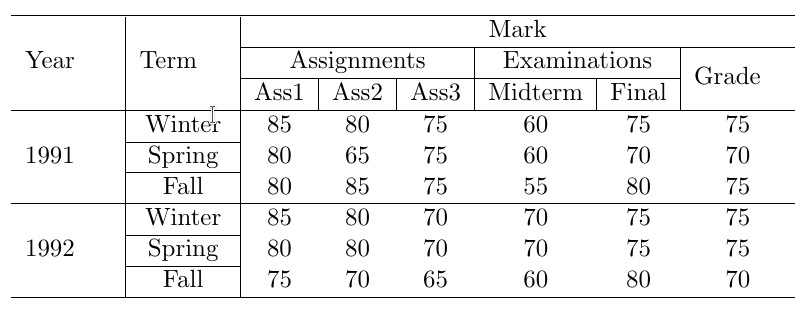
\includegraphics[width=0.8\textwidth]{img/tabel_verschillende_opstelling_dezelfde_data_1.png}
    \caption{Een tabel van evaluaties. Het geeft dezelfde informatie weer als tabelfiguur \ref{fig:tabel_verschillende_opstelling_dezelfde_data_2}. Bron: \cite{Long2010}}
    \label{fig:tabel_verschillende_opstelling_dezelfde_data_1}
\end{figure}

\begin{figure}[H]
    \centering
    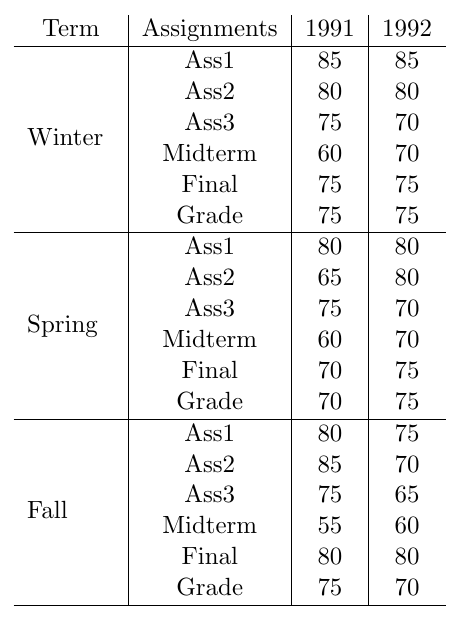
\includegraphics[width=0.5\textwidth]{img/tabel_verschillende_opstelling_dezelfde_data_2.png}
    \caption{Een tabel van evaluaties. Het geeft dezelfde informatie weer als tabelfiguur \ref{fig:tabel_verschillende_opstelling_dezelfde_data_1}. Bron: \cite{Long2010}}
    \label{fig:tabel_verschillende_opstelling_dezelfde_data_2}
\end{figure}

Hoewel beide tabellen identiek zijn wat informatieinhoud betreft, kan duidelijk gemerkt worden dat tabelfiguur \ref{fig:tabel_verschillende_opstelling_dezelfde_data_1} de evaluaties duidelijker weergeeft. Meestal wordt een combinatie van rijen en kolommen zodanig gekozen zodat de data van de tabel zo eenvoudig en snel mogelijk gelezen en geïnterpreteerd kan worden. Ook kunnen verschillende lettertypes, kleuren en lettergroottes gebruikt worden om de leesbaarheid te vergroten.

\subsection{Anatomie}
\label{subsec:anatomie}

\raggedbottom

Volgens \textcite{Wang1996} is een tabel, door \textit{stub scheiding} en \textit{boxhead scheiding}, verdeeld in vier hoofdregio's die in onderstaande figuur \ref{fig:tabel_anatomie} merkbaar zijn. De regio linksbeneden die de rijhoofdingen bevat en de regio rechtsboven die de kolomhoofdingen bevat, worden respectievelijk de \textit{stub} en de \textit{boxhead} genoemd. De regio linksboven, die de categorieën in de \textit{stub} inhouden is gekend als de \textit{stub head} en de \textit{body} tenslotte, is de regio rechts van de \textit{sub} en onder de \textit{boxhead} die de tabeldata-elementen bevat. De snijpunt van een rij en een kolom wordt een \textit{cel} genoemd; en een rechthoekig verzameling van \textit{cellen} is gekend als een \textit{block}.

\begin{figure}[H]
    \centering
    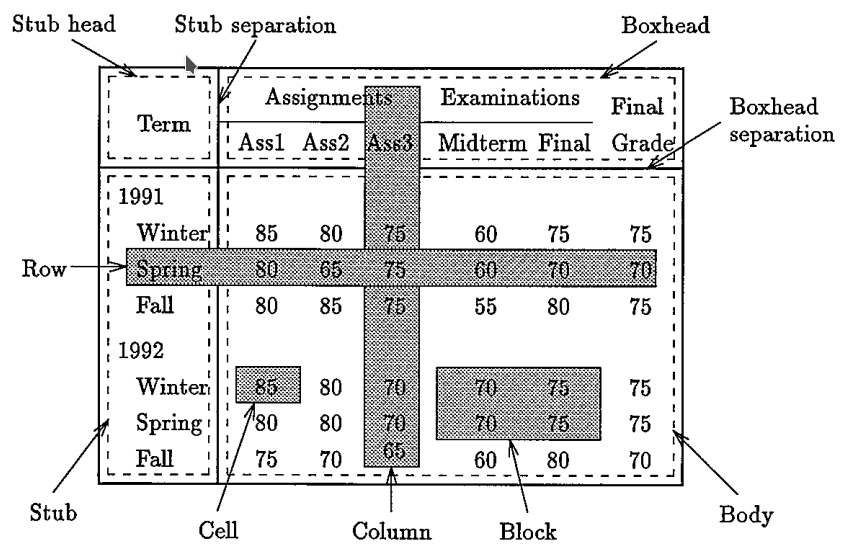
\includegraphics[width=0.8\textwidth]{img/tabel_anatomie.png}
    \caption{De anatomie van de structurele rij-kolomvoorstelling van een tabel. Bron: \cite{Wang1996}}
    \label{fig:tabel_anatomie}
\end{figure}

Zoals men in figuur \ref{fig:tabel_anatomie} kan zien, kunnen multidimensionele relaties in een twee dimensionele tabel gepresenteerd worden door meer dan één categorie te associeren met de \textit{boxhead} en/of met de \textit{stub}. Zo worden hier de rijhoofdingen niet enkel met één hoofdcategorie ``Term`` maar eveneens met meerdere subcategorieën, ``1991`` en ``1992`` geassocieerd. Analoog zijn de kolomhoofdingen gekoppeld aan drie categorieën, namelijk ``Assignments``, ``Examinations`` en ``Finals``.

\subsection{Creatie en representatie}
\label{subsec:creatie-en-representatie}

Doorheen de tijd werden verschillende software applicaties ontwikkeld om digitaal tabulair data aan te maken, te beheren en voor te stellen. Een veelgebruikte software voor tabelcompositie is Microsoft Excel. Het is, zoals \textcite{Wang1996} het vermeldt, een complexe rekenbladprogramma waarbij tabulair data in een werkblad, in een twee dimensionele rooster die a.d.h.v. rij en kolomindexes geadresseerd kan worden, geplaatst wordt.

Een andere bekend software voor het creëren van tabellen is \LaTeX. Het is een systeem voor het zetten van documenten. \textcite{Wang1996} geeft aan dat tabellen in \LaTeX\ gespecifieerd kunnen worden met de ``tabular``- en de ``array``-omgeving. De eerste omgeving wordt meestal gebruikt voor tekstuele tabeldata, de tweede voor wiskundige uitdrukkingen.

Voor de voorstelling van tabellen op het internet, m.a.w. op internetbrowsers, wordt de opmaaktaal HTML gebruikt. Door middel van de ``table``-, ``tr``-, ``th``- en ``td``-tags kunnen tabellen gemaakt en voorgesteld worden.

\section{Tabeldetectie}
\label{sec:tabel-detectie}

\subsection{Regelgebaseerde technieken}

\subsection{Datagedreven technieken}


\subsection{Performantieberekening}

\section{Tabelanalyse}
\label{sec:tabel-analyse}

\section{End-to-end-systemen}
\label{sec:end-to-end-systemen}
